% =========================================================================== %

\begin{frame}[t,plain]
\titlepage
\end{frame}

% =========================================================================== %

\begin{frame}{Recap}
%
\begin{columns}[T]
\column{.5\linewidth}
\begin{itemize}
\item tkInter: Basic logic
	\begin{itemize}
	\item All interactive objects: \enquote{widgets}
	\item Constructors set most properties
	\item Methods alter properties
	\item Widgets get \enquote{packed} in a main window
	\item Callback functions
	\end{itemize}
\item Packing
	\begin{itemize}
	\item Manually
	\item Frames
	\item Grids
	\item Combinations thereof
	\end{itemize}
\end{itemize}
%
\column{.5\linewidth}
\begin{itemize}
\item Variable mechanism
	\begin{itemize}
	\item Widgets with state
	\item Connected to a variable object
	\item In constructor: \texttt{variable = ...} or \texttt{textvariable = ...}
	\end{itemize}
\item Huge collection of objects
	\begin{itemize}
	\item Entries, TextBoxes
	\item CheckButtons, RadioButtons
	\item Pre-Built Dialogs
	\item Get used to look up things constantly
	\end{itemize}
\end{itemize}

\end{columns}
%
\begin{center}
	\emph{Any Questions?}
\end{center}
%
\end{frame}

% =========================================================================== %

\begin{frame}{Is It Worth the Time?}
%
\begin{columns}[T]
\column{.5\linewidth}
\includegraphics[width=\linewidth]{./gfx/xkcd-isItWorthTheTime}
%
\column{.5\linewidth}
\begin{center}
\emph{Don't forget the time you spend finding the chart to look up what you save. And the time spent reading this reminder about the time spent. And the time trying to figure out if either of those actually make sense. Remember, every second counts toward your life total, including these right now.}

\vspace{6pt}
Source: \url{https://xkcd.com/1205/}
\end{center}

\end{columns}
%
\end{frame}

% =========================================================================== %

\begin{frame}[fragile]{pandas -- Python data analysis toolkit}
%
\begin{itemize}
\item Toolkit for analyzing data in tables
\item Built upon NumPy and MatPlotLib
\item Comparable to R, SQL, Stata
\item Column and row-wise operations
\item Online documentation: \url{https://pandas.pydata.org/docs/user_guide/index.html}
\item PDF version: \url{https://pandas.pydata.org/docs/pandas.pdf} \\
	(3313 pages)
\item Needs to be installed first
\end{itemize}
%
\vspace{6pt}
\begin{tcbraster}[raster columns=2,
                  raster equal height,
                  nobeforeafter,
                  raster column skip=0.5cm]
\begin{cmdbox}[Installation: Anaconda]
\begin{minted}[fontsize=\scriptsize]{text}
conda install pandas
\end{minted}
\end{cmdbox}
%
\begin{cmdbox}[Installation: pip]
\begin{minted}[fontsize=\scriptsize]{text}
pip install pandas
\end{minted}
\end{cmdbox}
\end{tcbraster}
%
\end{frame}

% =========================================================================== %

\begin{frame}[fragile]{Convention}
%
\begin{center}
In any examples in this lecture, I will asume that these modules have been loaded with the symbols shown below.
\end{center}
%
\begin{codebox}[Implicitly: Import these modules]
\begin{minted}[linenos, fontsize=\scriptsize]{python3}
import pandas as pd
import numpy as np
import matplotlib.pyplot as plt
\end{minted}
\end{codebox}
%
\end{frame}

% =========================================================================== %

\begin{frame}[fragile]
%
\begin{columns}[T]
\column{.5\linewidth}
\begin{Large}
	{Elementary Object: Series}
	\vspace{6pt}
\end{Large}
\begin{itemize}
\item Represents one column of data
\item Comparable to NumPy array
\item All elements: same data type
\item Huge collection of convenience functions
\item New optional feature: index list, behaviour like \inPy{dict}s
\item Behaves like a NumPy array (slicing, boolean index lists, ...)
\item Supports \enquote{missing data}; represented as \texttt{NaN}
\end{itemize}
%
\column{.5\linewidth}
\begin{codebox}[Syntax: Creating a pandas Series]
\begin{minted}[fontsize=\scriptsize]{python3}
s = pd.Series(iterable)
s = pd.Series(iterable1, index=iterable2)
s = pd.Series(scalar, index=iterable)
s = pd.Series(dictionary)
\end{minted}
\end{codebox}
%
\begin{itemize}
\item New elements can be appended any time.
\item Arithmetic operations obey row alignment! If no match is found, the result is \inPy{None} (represented on screen as \texttt{NaN}.)
\end{itemize}
\end{columns}
%
\end{frame}

% =========================================================================== %

\begin{frame}[fragile]
%
\begin{tcbraster}[raster columns=2,
                  raster equal height,
                  nobeforeafter,
                  raster column skip=0.5cm]
\begin{codebox}[Example: pandas Series]
\begin{minted}[fontsize=\scriptsize, linenos]{python3}
print(
    pd.Series(np.arange(2, 0, -0.5)),
    "\n"
)

print( pd.Series("foo bar",
                 index=list("abcd")),
       "\n"
)

ser = pd.Series(np.arange(0, 2, +0.5),
                index=list("abcd"))
ser[0:3] = 420
ser['b'] = None
print(ser, "\n")

print(ser.a, ser["a"],
      ser.at["a"], ser.loc["a"]
      ser.iat[0], ser.iloc[0],
      ser.values[0])
\end{minted}
\end{codebox}
%
\begin{cmdbox}[Output: pandas Series]
\begin{minted}[fontsize=\scriptsize]{text}
0    2.0
1    1.5
2    1.0
3    0.5
dtype: float64

a    foo bar
b    foo bar
c    foo bar
d    foo bar
dtype: object

a    420.0
b      NaN
c    420.0
d      1.5
dtype: float64

420.0 420.0 420.0 420.0 420.0 420.0 420.0
\end{minted}
\end{cmdbox}
\end{tcbraster}
%
\end{frame}

% =========================================================================== %

\begin{frame}[fragile]
%
\begin{tcbraster}[raster columns=2,
                  raster equal height,
                  nobeforeafter,
                  raster column skip=0.5cm]
\begin{codebox}[Example: Series Addition]
\begin{minted}[fontsize=\scriptsize, linenos]{python3}
ser1 = pd.Series(
    np.arange(0, 2, +0.5),
    index=list("abcd")
)
ser2 = pd.Series(
    np.arange(2, 0, -0.5)
)
ser2['a'] = -1

ser3 = pd.Series(
    np.arange(2, 0, -0.5),
    index=list("abcd")
)

print(ser1 + ser2, "\n")
print(ser1 + ser3)
\end{minted}
\end{codebox}
%
\begin{cmdbox}[Output: Series Addition]
\begin{minted}[fontsize=\scriptsize]{text}
0    NaN
1    NaN
2    NaN
3    NaN
a   -1.0
b    NaN
c    NaN
d    NaN
dtype: float64

a    2.0
b    2.0
c    2.0
d    2.0
dtype: float64
\end{minted}
\end{cmdbox}
\end{tcbraster}
%
\end{frame}

% =========================================================================== %

\begin{frame}[fragile]
%
\begin{tcbraster}[raster columns=2,
                  raster equal height,
                  nobeforeafter,
                  raster column skip=0.5cm]
\begin{codebox}[Example: Useful Methods]
\begin{minted}[fontsize=\scriptsize, linenos]{python3}
ser  = pd.Series({
    chr(k + 65) : np.random.uniform()
    for k in range(5)
})

print( ser )
print()
print( "sum   :", ser.sum()
print( "prod  :", ser.prod() )
print( "median:", ser.median() )
print()
print( ser.describe() )
\end{minted}
\end{codebox}
%
\begin{cmdbox}[Output: Useful Methods]
\begin{minted}[fontsize=\scriptsize]{text}
A    0.951622
B    0.207435
C    0.287358
D    0.708257
E    0.176783
dtype: float64

sum   : 2.331453801556199
prod  : 0.0071023091881897635
median: 0.2873575745447944

count    5.000000
mean     0.466291
std      0.345301
min      0.176783
25%      0.207435
50%      0.287358
75%      0.708257
max      0.951622
dtype: float64
\end{minted}
\end{cmdbox}
%[0.9516216  0.20743477 0.28735757 0.70825697 0.17678289]
\end{tcbraster}
%
\end{frame}

% =========================================================================== %

\begin{frame}[fragile]
%
\begin{tcbraster}[raster columns=2,
                  raster equal height,
                  nobeforeafter,
                  raster column skip=0.5cm]
\begin{codebox}[Example: Boolean Array Indexing]
\begin{minted}[fontsize=\scriptsize, linenos]{python3}
ser  = pd.Series({
    chr( k + 65 ) : np.random.uniform()
    for k in range(4)
})

print( ser, "\n" )
ser[ ser > 0.5 ] = -ser
print( ser )
\end{minted}
\end{codebox}
%
\begin{cmdbox}[Output: Boolean Array Indexing]
\begin{minted}[fontsize=\scriptsize]{text}
A    0.733494
B    0.500153
C    0.160300
D    0.468744
dtype: float64 

A   -0.733494
B   -0.500153
C    0.160300
D    0.468744
dtype: float64
\end{minted}
\end{cmdbox}
\end{tcbraster}
%
\begin{hintbox}[SQL-Like Database Management]
\scriptsize
Line 7 of the above code translates to the SQL statement:
\begin{minted}[fontsize=\scriptsize]{SQL}
UPDATE ser
  SET content = -content
  WHERE content > 0.5;
\end{minted}
\end{hintbox}
%
\end{frame}

% =========================================================================== %

\begin{frame}[fragile]
%
\begin{tcbraster}[raster columns=2,
                  raster equal height,
                  nobeforeafter,
                  raster column skip=0.5cm]
\begin{codebox}[Example: Index updates and \texttt{reindex}]
\begin{minted}[fontsize=\scriptsize, linenos]{python3}
ser  = pd.Series({
    chr( k + 65 ) :
    np.random.randint(-5, 5)
    for k in range(4)
})

ser.index = list("abcd")
print(ser, "\n")

ser = ser.reindex(list("bada"))
print(ser, "\n")

print(ser["a"])
print(ser)
\end{minted}
\end{codebox}
%
\begin{cmdbox}[Output: Index updates and \texttt{reindex}]
\begin{minted}[fontsize=\scriptsize]{text}
a    1
b   -4
c   -4
d   -4
dtype: int64

b   -4
a    1
d   -4
a    1
dtype: int64

a    1
a    1
dtype: int64
\end{minted}
\end{cmdbox}
\end{tcbraster}
%
\end{frame}

% =========================================================================== %

\begin{frame}[fragile]{OneUp: DataFrames}
%
\begin{columns}[T]
\column{.5\linewidth}
%\begin{Large}
%	\vspace{6pt}
%\end{Large}
\begin{itemize}
\item Represents a \emph{table} of data
\item Collection of \texttt{pd.Series}
\item Comparable to NumPy 2D array
\item All \emph{data in a column}: same data type
\item Even larger collection of convenience functions than \texttt{pd.Series}
\item File IO support (CSV, JSON, Pickle, Excel/OpenDocument, SQL, SAS, SPSS, Clipboard, ...)
\end{itemize}
%
\column{.5\linewidth}
\begin{codebox}[Syntax: Creating a pandas DataFrame]
\begin{minted}[fontsize=\scriptsize]{python3}
s = pd.DataFrame(np_array_2D)
s = pd.DataFrame(np_array_2D,
                 index  = iterable1,
                 column = iterabel2
)
s = pd.DataFrame(scalar,
                 index  = iterable1,
                 column = iterabel2
)
s = pd.DataFrame(dict_key_Series)
...
\end{minted}
\end{codebox}
%
\end{columns}
%
\end{frame}

% =========================================================================== %

\begin{frame}{Available Data Formats}
%
\begin{center}
	\includegraphics[width=.75\linewidth]{./gfx/pandas-filecompat}
\end{center}
%
\scriptsize
From Chapter 2.4 in the documentation (IO Tools). The two rightmost columns are functions under \texttt{pd}, returning \texttt{pd.DataFrame}s.
%
\end{frame}

% =========================================================================== %

\begin{frame}{Data Source for Next Few Slides}
%
\begin{itemize}
\item CSV file: Pokémon up to Gen6
\item By GitHub user \emph{armgilles}
\item See Link\\
	{\scriptsize \url{https://gist.github.com/armgilles/194bcff35001e7eb53a2a8b441e8b2c6}}
\item Assume: File \texttt{pokemon.csv} in CWD
\end{itemize}
%
\begin{minipage}{.49\linewidth}
	\includegraphics[width=\linewidth]{./gfx/pokemon-csv}
\end{minipage}
%
\begin{minipage}{.49\linewidth}
	\includegraphics[width=\linewidth]{./gfx/pokemon-spreadsheet}
\end{minipage}
%
\end{frame}

% =========================================================================== %

\begin{frame}[fragile]
%
\begin{codebox}[Example: Reading a CSV and printing a \texttt{pd.DataFrame}]
\begin{minted}[linenos, fontsize=\scriptsize]{python3}
data = pd.read_csv("./pokemon.csv")
print(data)
\end{minted}
\end{codebox}
%
\begin{cmdbox}[Output: Reading a CSV and printing a \texttt{pd.DataFrame}]
\begin{minted}[fontsize=\scriptsize]{text}
       #                   Name   Type 1  ... Speed  Generation  Legendary
0      1              Bulbasaur    Grass  ...    45           1      False
1      2                Ivysaur    Grass  ...    60           1      False
2      3               Venusaur    Grass  ...    80           1      False
3      3  VenusaurMega Venusaur    Grass  ...    80           1      False
4      4             Charmander     Fire  ...    65           1      False
..   ...                    ...      ...  ...   ...         ...        ...
795  719                Diancie     Rock  ...    50           6       True
796  719    DiancieMega Diancie     Rock  ...   110           6       True
797  720    HoopaHoopa Confined  Psychic  ...    70           6       True
798  720     HoopaHoopa Unbound  Psychic  ...    80           6       True
799  721              Volcanion     Fire  ...    70           6       True

[800 rows x 13 columns]
\end{minted}
\end{cmdbox}
%
\end{frame}

% =========================================================================== %

\begin{frame}[fragile]
%
\begin{codebox}[Example: \texttt{set\_index} and column filtering]
\begin{minted}[linenos, firstnumber=3, fontsize=\scriptsize]{python3}
namedView = data.set_index("Name")
print(namedView[["HP", "Attack", "Defense"]])
\end{minted}
\end{codebox}
%
\begin{cmdbox}[Output: \texttt{set\_index} and column filtering]
\begin{minted}[fontsize=\scriptsize]{text}
                       HP  Attack  Defense
Name                                      
Bulbasaur              45      49       49
Ivysaur                60      62       63
Venusaur               80      82       83
VenusaurMega Venusaur  80     100      123
Charmander             39      52       43
...                    ..     ...      ...
Diancie                50     100      150
DiancieMega Diancie    50     160      110
HoopaHoopa Confined    80     110       60
HoopaHoopa Unbound     80     160       60
Volcanion              80     110      120

[800 rows x 3 columns]
\end{minted}
\end{cmdbox}
%
\end{frame}

% =========================================================================== %

\begin{frame}[fragile]
%
\begin{codebox}[Example: Adding New Columns]
\begin{minted}[linenos, firstnumber=5, fontsize=\scriptsize]{python3}
data["Offensive"] = data["Attack"]  + data["Sp. Atk"]
data["Defensive"] = data["Defense"] + data["Sp. Def"]

print(data     .head(2))      # likewise: df.tail(n)
print(namedView.head(2))
\end{minted}
\end{codebox}
%
\begin{cmdbox}[Output: Adding New Columns]
\begin{minted}[fontsize=\scriptsize]{text}
   #       Name Type 1  Type 2  ...  Generation  Legendary  Offensive  Defensive
0  1  Bulbasaur  Grass  Poison  ...           1      False        114        114
1  2    Ivysaur  Grass  Poison  ...           1      False        142        143

[2 rows x 15 columns]
           # Type 1  Type 2  Total  ...  Sp. Def  Speed  Generation  Legendary
Name                                ...                                       
Bulbasaur  1  Grass  Poison    318  ...       65     45           1      False
Ivysaur    2  Grass  Poison    405  ...       80     60           1      False

[2 rows x 12 columns]
\end{minted}
\end{cmdbox}
%
\end{frame}

% =========================================================================== %

\begin{frame}{Memory Modell}
%
\texttt{pd.DataFrame} only holds references to instances of \texttt{pd.Series}

\vspace{6pt}
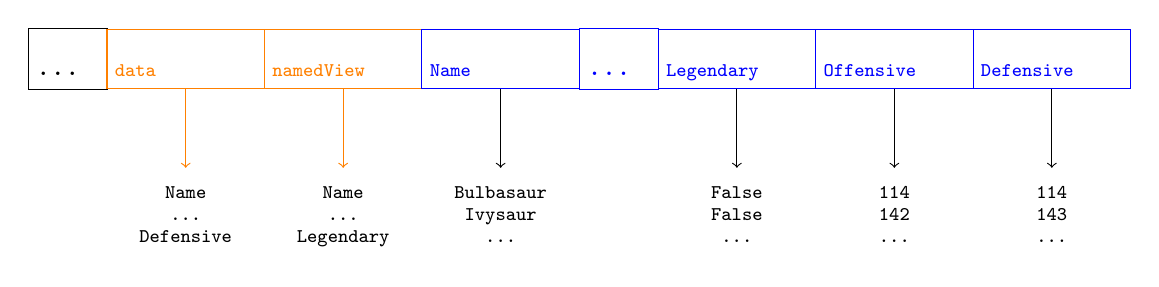
\begin{tikzpicture}
  [ 
    cell/.style={text width=18mm,
    text height=5mm, draw=black, inner sep=1mm},
    ld/.style={draw=orange,shorten >=2pt,->}
  ]
  
  \node (cElse)       at ( 0.0,0) [cell, text width=8mm] {\ttfamily \ldots\phantom{p}};
  \node (cDdata)      at ( 1.5,0) [cell, orange] {\ttfamily \scriptsize data \phantom{p}};
  \node (cDview)      at ( 3.5,0) [cell, orange] {\ttfamily \scriptsize namedView \phantom{p}};
  \node (cSname)      at ( 5.5,0) [cell, blue] {\ttfamily \scriptsize Name \phantom{p}};
  \node (cSelse)      at ( 7.0,0) [cell, blue, text width=8mm] {\ttfamily \ldots\phantom{p}};
  \node (cSlegendary) at ( 8.5,0) [cell, blue] {\ttfamily \scriptsize Legendary};
  \node (cSoffensive) at (10.5,0) [cell, blue] {\ttfamily \scriptsize Offensive \phantom{p}};
  \node (cSdefensive) at (12.5,0) [cell, blue] {\ttfamily \scriptsize Defensive \phantom{p}};
  
  \node (cTdata) at (1.5, -2.0) {\ttfamily \scriptsize 
	  \begin{tabular}{c}
	  Name \\
	  \ldots \\
	  Defensive
	  \end{tabular}
	};
  \node (cTview) at (3.5, -2.0) {\ttfamily \scriptsize 
	  \begin{tabular}{c}
	  		Name \\
	  		\ldots \\
	  		Legendary
	  \end{tabular}
  };
  \node (cTname) at (5.5, -2.0) {\ttfamily \scriptsize 
	  \begin{tabular}{c}
	  		Bulbasaur \\
	  		Ivysaur \\
	  		\ldots
	  \end{tabular}
  };
  \node (cTlegendary) at (8.5, -2.0) {\ttfamily \scriptsize 
	  \begin{tabular}{c}
	  		False \\
	  		False \\
	  		\ldots
	  \end{tabular}
  };
  \node (cToffensive) at (10.5, -2.0) {\ttfamily \scriptsize 
	  \begin{tabular}{c}
	  		114 \\
	  		142 \\
	  		\ldots
	  \end{tabular}
  };
  \node (cTdefensive) at (12.5, -2.0) {\ttfamily \scriptsize 
	  \begin{tabular}{c}
	  		114 \\
	  		143 \\
	  		\ldots
	  \end{tabular}
  };
  
  \draw [ld] (cDdata.south) -- (cTdata.north);
  \draw [ld] (cDview.south) -- (cTview.north);
  
  \draw [ld, draw=black] (cSname.south) -- (cTname.north);
  \draw [ld, draw=black] (cSlegendary.south) -- (cTlegendary.north);
  \draw [ld, draw=black] (cSoffensive.south) -- (cToffensive.north);
  \draw [ld, draw=black] (cSdefensive.south) -- (cTdefensive.north);
\end{tikzpicture}
\vspace{6pt}

Of course, \texttt{pd.Series} and \texttt{pd.DataFrame} have a method \texttt{copy}.
%
\end{frame}

% =========================================================================== %

\begin{frame}[fragile]
%
\begin{codebox}[Example: Extracting Unique Samples]
\begin{minted}[linenos, firstnumber=10, fontsize=\scriptsize]{python3}
print("All Types of Gen 1 Pokémon")
gen1View  = data[ data["Generation"] == 1]
gen1Types = pd.concat( [gen1View["Type 1"], gen1View["Type 2"]] ).dropna()
print(gen1Types.unique())
\end{minted}
\end{codebox}
%
\begin{cmdbox}[Output: Extracting Unique Samples]
\begin{minted}[fontsize=\scriptsize]{text}
All Types of Gen 1 Pokémon
['Grass' 'Fire' 'Water' 'Bug' 'Normal' 'Poison' 'Electric' 'Ground' 'Fairy' 'Fighting'
 'Psychic' 'Rock' 'Ghost' 'Ice' 'Dragon' 'Flying' 'Steel' 'Dark']
\end{minted}
\end{cmdbox}
%
\begin{hintbox}[SQL-Like Database Management]
\scriptsize
\begin{minted}[fontsize=\scriptsize]{SQL}
SELECT DISTINCT * AS content FROM
   SELECT Type_1 FROM data WHERE Generation == 1
   UNION
   SELECT Type_2 FROM data WHERE Generation == 1
WHERE content NOT NULL;
\end{minted}
\end{hintbox}
%
\end{frame}

% =========================================================================== %

\begin{frame}{Grouping and Sorting}
%
\begin{columns}[T]
\column{.5\linewidth}
Grouping
\begin{itemize}
\item Method \texttt{groupby}
\item Takes column name or list of column names
\item Returns reference to original DataFrame
\item Allows \emph{aggregate functions} as methods
	\begin{itemize}
	\item \texttt{mean}, \texttt{median}, \texttt{min}, \texttt{max}, \texttt{sum}, \texttt{count}, ...
	\item Method \texttt{aggregate}: pass arbitrary reduction function
	\end{itemize}
\item Aggregated Group-Object can be used like a DataFrame
\end{itemize}
%
\column{.5\linewidth}
Sorting
\begin{itemize}
\item Functions \texttt{sort\_values} and \texttt{sort\_index}
\item Parameter: Column name or list of column names
\item Optional: \texttt{ascending=False}
\item Optional: \texttt{inplace=True}
\end{itemize}
\end{columns}
%
\end{frame}

% =========================================================================== %

\begin{frame}[fragile]
%
\begin{codebox}[Example: Grouping{,} Sorting and Aggregates]
\begin{minted}[linenos, firstnumber=14, fontsize=\scriptsize]{python3}
groupedByType1 = namedView.groupby("Type 1")
groupMeans = groupedByType1.mean().sort_values("Total", ascending=False)
print(groupMeans.head(10))
\end{minted}
\end{codebox}
%
\begin{cmdbox}[Output: Grouping{,} Sorting  and Aggregates]
\begin{minted}[fontsize=\scriptsize]{text}
                   #       Total         HP  ...       Speed  Generation  Legendary
Type 1                                       ...                                   
Dragon    474.375000  550.531250  83.312500  ...   83.031250    3.875000   0.375000
Steel     442.851852  487.703704  65.222222  ...   55.259259    3.851852   0.148148
Flying    677.750000  485.000000  70.750000  ...  102.500000    5.500000   0.500000
Psychic   380.807018  475.947368  70.631579  ...   81.491228    3.385965   0.245614
Fire      327.403846  458.076923  69.903846  ...   74.442308    3.211538   0.096154
Rock      392.727273  453.750000  65.363636  ...   55.909091    3.454545   0.090909
Dark      461.354839  445.741935  66.806452  ...   76.161290    4.032258   0.064516
Electric  363.500000  443.409091  59.795455  ...   84.500000    3.272727   0.090909
Ghost     486.500000  439.562500  64.437500  ...   64.343750    4.187500   0.062500
Ground    356.281250  437.500000  73.781250  ...   63.906250    3.156250   0.125000
\end{minted}
\end{cmdbox}
%
\end{frame}

% =========================================================================== %

\begin{frame}[fragile]
%
\begin{codebox}[Example: Grouping{,} Sorting and Aggregates]
\begin{minted}[linenos, firstnumber=14, fontsize=\scriptsize]{python3}
relMeanDeviation = lambda x : (x - np.mean(x)) / np.mean(x)
cols = data.columns[4:]   # all non-string columns

relativeData = data[cols].transform(relMeanDeviation)

print(relativeData.head(5))
\end{minted}
\end{codebox}
%
\begin{cmdbox}[Output: Grouping{,} Sorting  and Aggregates]
\begin{minted}[fontsize=\scriptsize]{text}
      Total        HP    Attack  ...  Legendary  Offensive  Defensive
0 -0.269138 -0.350263 -0.379757  ...       -1.0  -0.249117  -0.217812
1 -0.069185 -0.133683 -0.215202  ...       -1.0  -0.064690  -0.018834
2  0.206612  0.155089  0.037958  ...       -1.0   0.198778   0.255618
3  0.436443  0.155089  0.265803  ...       -1.0   0.462246   0.667296
4 -0.289823 -0.436894 -0.341783  ...       -1.0  -0.262290  -0.361899

[5 rows x 11 columns]
\end{minted}
\end{cmdbox}
%
\end{frame}

% =========================================================================== %

\begin{frame}{Binning}
%
\begin{itemize}
\item Classify DataFrame by continuous numerical value
\item E.\;g. HP between 100 and 120
\item Function \texttt{pd.cut}
	\begin{itemize}
	\item Takes a \texttt{pd.Series}, and a list of boundary values
	\item E.\;g.: \texttt{[1, 2, 4]} $\thus ~ (-\infty, 1], (1, 2], (2, 4], (4, +\infty)$
	\item Returns a \emph{Categories object}
	\end{itemize}
\item A \emph{Categories object}
	\begin{itemize}
	\item Essentially: Assignment \emph{line in DataFrame} \thus~ \emph{bin}
	\item Also: Bin Size, \eg $(2, 4]$
	\item Internally: \texttt{pd.Series}
	\end{itemize}
\end{itemize}
%
\end{frame}

% =========================================================================== %

\begin{frame}[fragile]
%
\begin{codebox}[Example: Binning]
\begin{minted}[linenos, firstnumber=20, fontsize=\scriptsize]{python3}
boundaries = np.linspace( data.Total.min(), data.Total.max(), 11 )
bins = pd.cut(namedView["Total"], boundaries)

print("Charizard is in bin: ", bins["Charizard"])
print("Pokémon in the same bin:")
print(namedView[bins == bins["Charizard"]].index)
\end{minted}
\end{codebox}
%
\begin{cmdbox}[Output: Binning]
\begin{minted}[fontsize=\scriptsize]{text}
Charizard is in bin:  (480.0, 540.0]
Pokémon in the same bin:
Index(['Venusaur', 'Charizard', 'Blastoise', 'BeedrillMega Beedrill', 'Raichu',
       'Nidoqueen', 'Nidoking', 'Clefable', 'Ninetales', 'Vileplume',
       ...
       'Aurorus', 'Sylveon', 'Hawlucha', 'Carbink', 'GourgeistAverage Size',
       'GourgeistSmall Size', 'GourgeistLarge Size', 'GourgeistSuper Size',
       'Avalugg', 'Noivern'],
      dtype='object', name='Name', length=192)
\end{minted}
\end{cmdbox}
%
\end{frame}

% =========================================================================== %

\begin{frame}{Iterating over DataFrames}
%
\begin{columns}[T]
\column{.5\linewidth}
\begin{itemize}
\item \inPy{for col in df : ...}
	\begin{itemize}
	\item Get all column-heads (\eg \texttt{"HP"}, \texttt{"Attack"}, \ldots)
	\item \inPy{type(col)} as specified when creating the DataFrame; usually \inPy{str}ing
	\end{itemize}
\item \inPy{for col in df.iteritems() : ...}
	\begin{itemize}
	\item Get all columns as Series (\eg \texttt{"Charmander"}, \texttt{"Charmeleon"}, \ldots)
	\item \inPy{type(col) == tuple}: \texttt{(column-index, pd.Series)}
	\end{itemize}
\end{itemize}
%
\column{.5\linewidth}
\begin{itemize}
\item \inPy{for row in df.iterrows() : ...}
	\begin{itemize}
	\item Get all rows as Series
	\item Index of Series: Column in DataFrame
	\item Value: according to row
	\item \inPy{type(row) == tuple}: \texttt{(row-index, pd.Series)}
	\end{itemize}
\item \inPy{for row in df.itertuples() }
	\begin{itemize}
	\item Like \texttt{iterrows}, different output type
	\item \inPy{type(row) == pd.Pandas}, behaves like a \inPy{tuple}
	\item \texttt{(row-index, value1, value2, ...)}
	\end{itemize}
\end{itemize}
\end{columns}
%
\end{frame}

% =========================================================================== %

\begin{frame}[fragile]
%
\begin{tcbraster}[raster columns=2,
                  raster equal height,
                  nobeforeafter,
                  raster column skip=0.5cm]
\begin{codebox}[Example: Loop over DataFrame]
\begin{minted}[fontsize=\scriptsize, linenos, firstnumber=26]{python3}
for x in data :
    print(x)
\end{minted}
\end{codebox}
%
\begin{codebox}[Example: Loop over \texttt{iteritems}]
\begin{minted}[fontsize=\scriptsize, linenos, firstnumber=28]{python3}
for x in data.iteritems() :
    print(x)
\end{minted}
\end{codebox}
\end{tcbraster}
%
\begin{tcbraster}[raster columns=2,
                  raster equal height,
                  nobeforeafter,
                  raster column skip=0.5cm]
\begin{cmdbox}[Output: Loop over DataFrame]
\begin{minted}[fontsize=\scriptsize]{text}
#
Name
Type 1
Type 2
Total
HP
Attack
Defense
Sp. Atk
Sp. Def
Speed
Generation
Legendary
\end{minted}
\end{cmdbox}
%
\begin{cmdbox}[Output: Loop over \texttt{iteritems}]
\begin{minted}[fontsize=\scriptsize]{text}
...
('Name', 0                  Bulbasaur
1                    Ivysaur
2                   Venusaur
3      VenusaurMega Venusaur
4                 Charmander
               ...          
795                  Diancie
796      DiancieMega Diancie
797      HoopaHoopa Confined
798       HoopaHoopa Unbound
799                Volcanion
Name: Name, Length: 800, dtype: object)
...
\end{minted}
\end{cmdbox}
\end{tcbraster}
%
\end{frame}

% =========================================================================== %

\begin{frame}[fragile]
%
\begin{tcbraster}[raster columns=2,
                  raster equal height,
                  nobeforeafter,
                  raster column skip=0.5cm]
\begin{codebox}[Example: Loop over \texttt{iterrows}]
\begin{minted}[fontsize=\scriptsize, linenos, firstnumber=30]{python3}
for x in data.iterrows() :
    print(x)
\end{minted}
\end{codebox}
%
\begin{codebox}[Example: Loop over \texttt{itertuples}]
\begin{minted}[fontsize=\scriptsize, linenos, firstnumber=32]{python3}
for x in data.itertuples() :
    print(x)
\end{minted}
\end{codebox}
\end{tcbraster}
%
\begin{tcbraster}[raster columns=2,
                  raster equal height,
                  nobeforeafter,
                  raster column skip=0.5cm]
\begin{cmdbox}[Output: Loop over \texttt{iterrows}]
\begin{minted}[fontsize=\scriptsize]{text}
(0, #                     1
Name          Bulbasaur
Type 1            Grass
Type 2           Poison
Total               318
HP                   45
Attack               49
Defense              49
Sp. Atk              65
Sp. Def              65
Speed                45
Generation            1
Legendary         False
Name: 0, dtype: object)
\end{minted}
\end{cmdbox}
%
\begin{cmdbox}[Output: Loop over \texttt{itertuples}]
\begin{minted}[fontsize=\scriptsize]{text}
Pandas(Index=0, _1=1, Name='Bulbasaur',
       _3='Grass', _4='Poison',
       Total=318, HP=45, Attack=49,
       Defense=49, _9=65, _10=65,
       Speed=45, Generation=1,
       Legendary=False)
\end{minted}
\end{cmdbox}
\end{tcbraster}
%
\end{frame}

% =========================================================================== %

\begin{frame}{Plotting}
%
\begin{itemize}
\item Direct connection to MatPlotLib exists
\item Simply do \texttt{ser.plot()} -- get an \texttt{plt.Axis} object
\item Follow up \texttt{plt.show()} -- done
\item \texttt{plot} is actually directly from MatPlotLib and takes the same optional arguments
	\begin{itemize}
	\item \eg \texttt{ser.plot(linestyle="", marker=".")}
	\item Makes a scatterplot instead of a line plot
	\end{itemize}
\item \texttt{ser.plot.bar()}, \texttt{ser.plot.barh()}, \texttt{ser.plot.hist()}, ...
\item Works also with DataFrames -- plots each Series as an individual line
\end{itemize}
%
\end{frame}

% =========================================================================== %

\begin{frame}[fragile]
%
\begin{columns}[T]
\column{.5\linewidth}
\begin{codebox}[Syntax: Title goes here]
\begin{minted}[fontsize=\scriptsize, linenos, firstnumber=34]{python3}
data["Attack"].plot()
plt.xlabel("Pokémon ID")
plt.ylabel("Attack")
plt.show()
\end{minted}
\end{codebox}
%
\begin{center}
	\includegraphics[width=.8\linewidth]{./gfx/pokemon-atk}
\end{center}
%
\column{.5\linewidth}
\begin{codebox}[Syntax: Title goes here]
\begin{minted}[fontsize=\scriptsize, linenos, firstnumber=38]{python3}
data.plot()
plt.xlabel("Pokémon ID")
plt.ylabel("Status")
plt.show()
\end{minted}
\end{codebox}
%
\begin{center}
	\includegraphics[width=.8\linewidth]{./gfx/pokemon-tot}
\end{center}
\end{columns}
%
\end{frame}

% =========================================================================== %

\begin{frame}{Plus Ultra}
%
\begin{columns}[T]
\column{.5\linewidth}
\begin{itemize}
\item Dateseries
\item Pivot Tables
\item Rolling Windows
\item Inner and Outer Joins
\end{itemize}
%
\column{.5\linewidth}
\begin{itemize}
\item Tools for working with text
\item Removal of duplicates
\item Formatted output (HTML)
\item Random Samples
\end{itemize}
\end{columns}

\vspace{12pt}
\begin{center}
\emph{You FOOL! This isnt even my final form! Wait until you see my TRUE power! HYAAAAAAAAAAAAAAAA!}
\end{center}
\begin{flushright}
\scriptsize
Frieza, Dragon Ball Z
\end{flushright}
%
%\begin{hintbox}[A Language of its Own]
%Given that pandas builds upon two other modules and offers so much functionality, you can think of it as a database language in itself, much like SQL or R which it attempts to emulate.
%\end{hintbox}
%
\end{frame}
